\documentclass[12pt]{report}

\usepackage{scribe_MG}

\usepackage[english]{babel}
\usepackage[utf8x]{inputenc}
\usepackage[T1]{fontenc}

\usepackage{amsmath}
\usepackage{amssymb}
\usepackage{graphicx}
\usepackage[colorinlistoftodos]{todonotes}
\usepackage[colorlinks=true, allcolors=blue]{hyperref}

\usepackage{tikz}
\usetikzlibrary{positioning}

\begin{document}
\coursetitle{IFT 6269: Probabilistic Graphical Models}
\semester{Fall 2017}
\lecturer{Simon Lacoste-Julien} \scribe{Isabela Albuquerque}
\lecturenumber{1} \lecturedate{September 5}

\maketitle

\section{Probabilistic Graphical Models}
\begin{itemize}
\item Goal: Model multivariate data
\item Mix of graph and probability theory. Or, more illustratively:
\begin{figure}[h]
\centering
\includegraphics[width=0.4\textwidth]{VennGM.png}
\end{figure}

\item Probability vs. Statistics:

\begin{center}
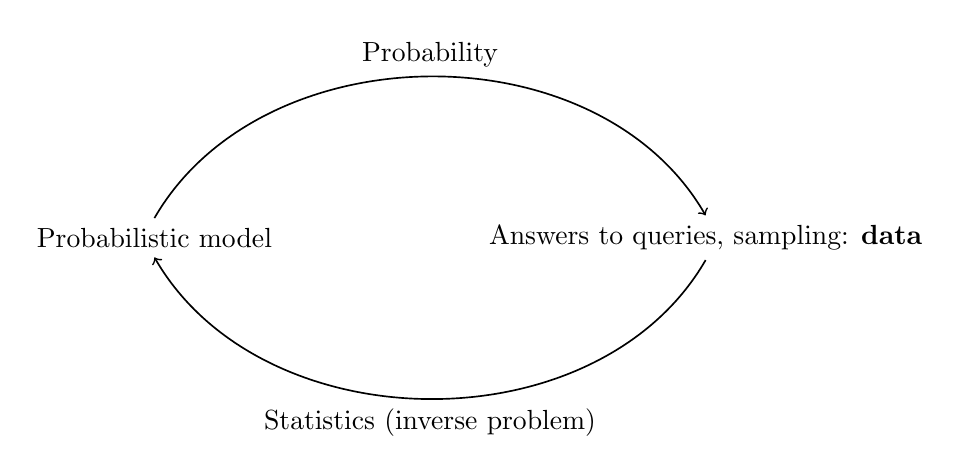
\begin{tikzpicture}[-latex, auto, node distance = 7cm and 7cm, on grid, semithick,
state/.style ={circle, top color = white, draw, text = black, minimum width=2.5cm}]
\node (A) {Probabilistic model};
\node (B) [right = of A] {Answers to queries, sampling: \textbf{data}};
       
\draw [->, out=60, in=120] (A.north) to node[above]{Probability}  (B.north);
\draw [->, out=-120, in=-60] (B.south) to node[below]{Statistics (inverse problem)} (A.south);
\end{tikzpicture}
\end{center}
\end{itemize}

\section{Applications}
Some illustrative examples of Hidden Markov Models (HMM) applications. \\ 

\noindent\fbox{%
    \parbox{\textwidth}{%
        \textit{Notation:}
\begin{itemize}
\item[-] $X_t$: \textbf{Observed} random variable. Represented in the graphical model as a \textbf{shaded} node.
\item[-] $Y_t$: \textbf{Not observed} random variable. Represented in the graphical model as an \textbf{empty} node.	
\item[-] Graph edges ($-$): Represents possible correlations between random variables in the graphical models. Lack of edges in the graph will represent \textbf{conditional independence} assumptions, as we will see later.
\end{itemize}
    }%
} \\
\newline \textcolor{red}{
\textit{Important!}
\begin{itemize}
\item[-] When modeling a problem using graphical models, random variables represent the quantities of interest.
\item[-] In the context of PGM, a random vector is often just called a \emph{random variable} -- thus a random variable might be scalar or vector valued.
\end{itemize}
}

\subsection{Example 1: Speech Recognition}
$X_t$: Sound wave encoding for a small time window (e.g. as a spectral decomposition) \\
$Y_t$: Phoneme
\begin{center}
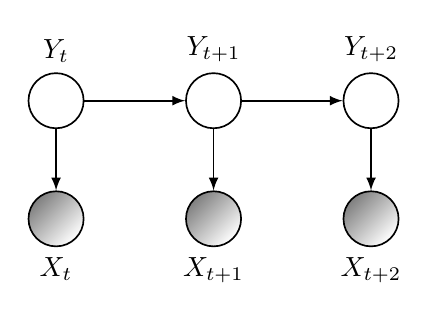
\begin{tikzpicture}[-latex, auto, node distance = 1.5cm and 2cm, on grid, semithick,
state/.style ={circle, top color = white, draw, text = black, minimum width=0.7cm}, sh/.style={shade, shading = axis, left color = gray, shading angle = 45}]
\node[state, label = above:{$Y_t$}] (A) {};
\node[state, label = above:{$Y_{t+1}$}] (B) [right = of A] {};
\node[state, label = above:{$Y_{t+2}$}] (C) [right = of B] {};
\node[state, label = below:{$X_t$}] (D) [below = of A] [sh] {};
\node[state, label = below:{$X_{t+1}$}] (E) [right = of D] [sh] {};
\node[state, label = below:{$X_{t+2}$}] (F) [right = of E] [sh] {};
\path (A) edge node {} (D)
		  edge node {} (B)
	  (B) edge node {} (E)
		  edge node {} (C)
	  (C) edge node {} (F);          
\end{tikzpicture}
\end{center}

\subsection{Example 2: Part-of-speech tagging}
$X_t$: Word \\
$Y_t$: Part-of-speech (word grammatical classification)
\begin{center}
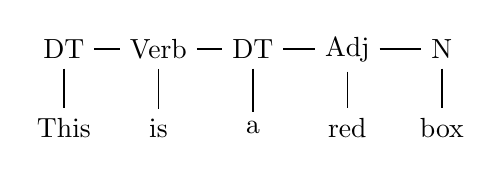
\begin{tikzpicture}[-latex, auto, node distance = 1cm and 1.2cm, on grid, semithick,
state/.style ={circle, top color = white, draw, text = black, minimum width=1.2cm}]
\node (A) {DT};
\node (B) [right = of A] {Verb};
\node (C) [right = of B] {DT};
\node (D) [right = of C] {Adj};
\node (E) [right = of D] {N};
\node (F) [below = of A] {This};
\node (G) [right = of F] {is};
\node (H) [right = of G] {a};
\node (I) [right = of H] {red};
\node (J) [right = of I] {box};

\path[-] (A) edge node {} (F)
		     edge node {} (B)
	     (B) edge node {} (G)
		     edge node {} (C)
	     (C) edge node {} (H)
             edge node {} (D)
		 (D) edge node {} (I)
	         edge node {} (E)
         (E) edge node {} (J);          
\end{tikzpicture}
\end{center}

\subsection{Example 3: Gene finding}
$X_t$: Sequence of nitrogenous base \\
$Y_t$: Coding or non-coding (i.e. $Y_t \in \{0;1\}$)

\begin{center}
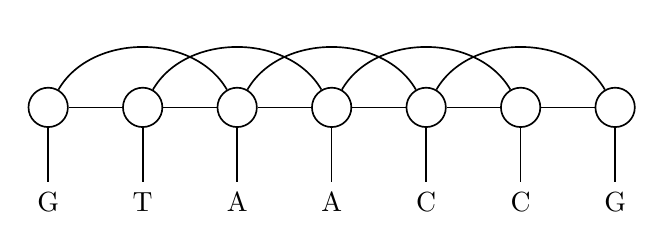
\begin{tikzpicture}[-latex, auto, node distance = 1.2cm and 1.2cm, on grid, semithick,
state/.style ={circle, top color = white, draw, text = black, minimum width=0.5cm}]
\node[state] (A) {};
\node[state] (B) [right = of A] {};
\node[state] (C) [right = of B] {};
\node[state] (D) [right = of C] {};
\node[state] (E) [right = of D] {};
\node[state] (F) [right = of E] {};
\node[state] (G) [right = of F] {};
\node (I) [below = of A] {G};
\node (J) [right = of I] {T};
\node (K) [right = of J] {A};
\node (L) [right = of K] {A};
\node (M) [right = of L] {C};
\node (N) [right = of M] {C};
\node (O) [right = of N] {G};

\path[-] (A) edge node {} (B)
			 edge node {} (I)
             edge [bend left = 60] node {} (C)
		 (B) edge node {} (C)
             edge node {} (J)
             edge [bend left = 60] node {} (D)
         (C) edge node {} (D)
             edge node {} (K)
             edge [bend left = 60] node {} (E)
         (D) edge node {} (E)
             edge node {} (L)
             edge [bend left = 60] node {} (F)
         (E) edge node {} (F)
             edge node {} (M)
             edge [bend left = 60] node {} (G)
         (F) edge node {} (G)
             edge node {} (N)
         (G) edge node {} (O);     
\end{tikzpicture}
\end{center}

\subsection{Example 4: Control system}
\begin{equation*}
\begin{split}
&y_{t+1} = A y_t + B v_t + \epsilon_t, \qquad \textcolor{blue}{\text{($y_t$ is the latent state)}} \\
& x_t = C y_t + \epsilon'_{t}, \qquad \qquad \qquad \textcolor{blue}{\text{(Observation)}}
\end{split}
\end{equation*}
where $y_t$ and $x_t$ are continuous vectors and $v_t$ is a given control term. The terms $\epsilon$ and $\epsilon'$ represent the noise in the system. If they are modeled as Gaussian noise, this HMM is a Kalman Filter. \\

\section{Why Graphical Models?}
Back to the part-of-speech tagging example: \\

\noindent\fbox{%
    \parbox{\textwidth}{%
\textit{Notation:}
\begin{itemize}
\item[-] An observation of $T$ words is represented as $( x_1, x_2, \ldots, x_T) \triangleq x_{1:T}$ 
\item[-] For a vocabulary of size $k$, $x_t \in \{1, \ldots, k \}$  
\end{itemize}
	}
}
\\ 
\newline \textit{Problem:} We want to model $p(x_{1:T})$, which corresponds to an exponential size state space. Thus, $\approx K^T$ parameters have to be estimated to define a probability distribution on $x_{1:T}$ \\
\newline \textcolor{violet}{Trick: make a factorization assumption about the distribution $p(x_{1:T})$.
\begin{equation*}
p(x_1, \ldots, x_T) = f_1(x_1)f_2(x_2|x_1)f_3(x_3|x_2) \ldots f_T(x_T|x_{T-1}).
\end{equation*}
Each factor $f$ can be seen as a clique in the graphical model and needs $\approx K^2$ parameters to be specified. As we have T factors in this factorization, we reduce the total number of parameters from $K^T$ (exponentially grows with $T$) to $TK^2$ (linearly grows with $T$).
} \\
\newline Now, back to our problem, say we want to compute the marginal probability of $x_1$, $p(x_1) = \displaystyle\sum_{x_2, \ldots, x_T} p(x_{1:T})$. Using the factorization assumption, we can write $p(x_1)$ as:
\begin{equation}
\label{factorization}
p(x_1) = \sum_{x_2, \ldots, x_T} f_1(x_1)f_2(x_2|x_1)f_3(x_3|x_2) \ldots f_T(x_T|x_{T-1}).
\end{equation}

\noindent Applying the distributive property of the product over a sum ($a(b+c) = ab + ac$), we can rewrite equation \ref{factorization} as

\begin{equation}
p(x_1) = f_1(x_1) \left( \sum_{x_2}f_2(x_2|x_1) \left( \sum_{x_3} f_3(x_3|x_2) \ldots \left( \sum_{x_T} f_T(x_T|x_{T-1}) \right) \ldots \right) \right).
\end{equation}

\noindent This organized and efficient way to compute the marginal $p(x_1)$ is known as the \textbf{Message passing algorithm}. The term $\displaystyle\sum_{x_T} f_T(x_T|x_{T-1})$ is named message and denoted as $M_{T}(x_{T-1})$. The following figure illustrates $M_{T}(x_{T-1})$ (represented by the red arrow) passing through a graph.

\begin{center}
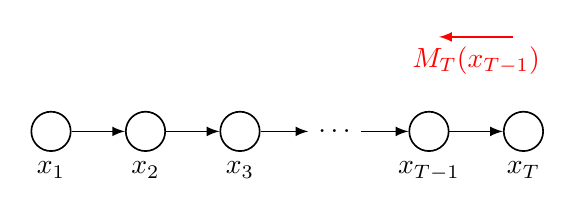
\begin{tikzpicture}[-latex, auto, node distance = 1.2cm and 1.2cm, on grid, semithick,
state/.style ={circle, top color = white, draw, text = black, minimum width = 0.5cm}]
\node[state, label = below:{$x_1$}] (A) {};
\node[state, label = below:{$x_2$}] (B) [right = of A] {};
\node[state, label = below:{$x_3$}] (C) [right = of B] {};
\node (D) [right = of C] {$\ldots$};
\node[state, label = below:{$x_{T-1}$}] (E) [right = of D] {};
\node[state, label = below:{$x_T$}] (F) [right = of E] {};
\node (G) [above = of F] {};
\node (H) [above = of E] {};

\path (A) edge node {} (B)
	  (B) edge node {} (C)
      (C) edge node {} (D)
      (D) edge node {} (E)
      (E) edge node {} (F);
\path[red] (G) edge node {$M_T(x_{T-1})$} (H);   
\end{tikzpicture}
\end{center}

\section{Key Themes}
\begin{enumerate}
\item Representation: how to represent structured probability distributions.
\begin{itemize}
\item[-] Related to parameterization (\textit{e.g.} full table, exponential family) 
\end{itemize}
\item Estimation: given data samples, how do we learn the parameters of the distribution underlying the observations?
\begin{itemize}
\item[-] Related to learning (\textit{e.g.} Maximum Likelihood Estimation) 
\end{itemize}
\item Inference: answer questions about the data, as computing conditional distributions $p(y|x)$ or marginals $p(x_1)$.
\begin{itemize}
\item[-] Efficient computation (\textit{e.g.} Message passing algorithm) 
\end{itemize}
\end{enumerate}
\end{document}